\documentclass[12pt]{article}

% Page setup
\usepackage[a4paper, margin=1in]{geometry}

% Math packages
\usepackage{amsmath, amssymb, amsfonts}
\usepackage{mathtools}
\usepackage{bm}          % bold math symbols
\usepackage{graphicx}
\usepackage{subcaption}

% Spacing
\usepackage{setspace}
\onehalfspacing
\setlength{\parindent}{0pt}
\setlength{\parskip}{6pt}

% Theorem environments
\usepackage{amsthm}
\newtheorem{definition}{Definition}
\newtheorem{theorem}{Theorem}
\newtheorem{lemma}{Lemma}
\newtheorem{proposition}{Proposition}

% Custom commands
\newcommand{\R}{\mathbb{R}}
\newcommand{\X}{\bm{X}}
\newcommand{\x}{\bm{x}}
\newcommand{\w}{\bm{w}}
\newcommand{\muvec}{\bm{\mu}}
\newcommand{\SigmaMat}{\bm{\Sigma}}

\numberwithin{equation}{section}

\begin{document}
\begin{center}
    {\LARGE \textbf{Independent Component Analysis}}\\[4pt]
    {\large Mathematical Derivation}\\
    {\small Notes by Muskaan Saxena}
\end{center}
\vspace{10pt}

% =========================
\section*{Introduction to Blind Source Separation}

\textbf{Problem Formulation:} \\
Consider a room with 3 people talking, there are 3 microphones placed at different locations in the room. Each of them record the 3 speakers, some of them will capture, lets say speaker 1 more prominently and others might capture more of the other speaker's voice. This is known as the cocktail party problem.

Blind Source Separation (BSS) is a computational technique that aims to extract individual source signals from a mixture when nothing is known about the way they were combined.

BSS Algorithms analyze statistical properties of the mixed signals to identify patterns that allow separation. One such algorithm is Independent Component Analysis (ICA).

\section*{Independent Component Analysis (ICA)} 

It is a technique used to separate mixed signals into their independent, non-Gaussian components. It aims to find a linear transformation of data that maximizes statistical independence among the components.

The mathematical formulation of ICA is given in the form of a statistical estimation problem. \\

\textbf{Assumptions:}
\begin{itemize}
    \item The source signals are statistically independent of each other.
     \[
     P(X \cap Y) = P(X) P(Y)
     \]
     \item The source signals have Non-Gaussian distributions.
\end{itemize}

\textbf{Objective:} \\
To decompose signal mixtures into \textbf{independent} and \textbf{maximally 'Non-Gaussian' sources}.

\section*{Mixing Model}
say, the observed signals (mixtures) are the vectors $\x(t) = \x_i = \x_1, \x_2, \x_3 \dots \x_n$

Where t = time index

Each of these is a weighted sum of the speech signals emitted by the 3 speakers, $s_1(t), s_2(t)$ and $s_3(t)$.
\[
\x(t) = A . s
\]

where $A =$ mixing matrix, $s =$ latent sources and $\x =$ observations. \[
A = \begin{bmatrix}
    a_{11} & a_{12} & a_{13} \\
    a_{21} & a_{22} & a_{23}\\
    a_{31} & a_{32} & a_{33}\\
\end{bmatrix}
\quad \text{and} \quad
s = \begin{bmatrix}
    s_1 \\
    s_2 \\
    s_3
\end{bmatrix}
\]
so,

\[\x_i = \begin{bmatrix}
a_{11}s_1 + \dots + a_{1m}s_m \\
a_{21}s_1 + \dots + a_{2m}s_m \\
\vdots \\
a_{n1}s_1 + \dots + a_{nm}s_m 
\end{bmatrix}
\]

Where $n =$ number of observed time courses \\
$m =$ number of latent sources \\
and $k =$ number of time samples. \\

\[
\begin{aligned}
A &\in \mathbb{R}^{n \times m} \\
\x &\in \mathbb{R}^{n \times k} \\
s &\in \mathbb{R}^{m \times k}
\end{aligned}
\]

so, considering 3 people it becomes: 

\begin{align*}
    \x_1(t) = a_{11} s_1(t) + a_{12} s_2(t) +a_{13}s_3(t)\\
    \x_2(t) = a_{21}s_1(t) + a_{22}s_2(t) + a_{23}s_3(t)\\
    \x_3(t) = a_{31}s_1(t) + a_{32}s_2(t) + a_{33}s_3(t)\\
\end{align*}

\textbf{Mixing Model Assumptions:}
\begin{itemize}
    \item Neither mixing matrix $A$ nor sources $s$ are known, we assume that all sources have unit variance.
    \item We accept any ordering or ranking of sources since any permutation yields the same observations.
    \item We assume that mixing matrix is square and orthogonal i.e. the number of independent sources is equal to the number of observations.\\
\end{itemize} 

\begin{figure}[h]
    \centering

    \begin{subfigure}{0.45\textwidth}
        \centering
        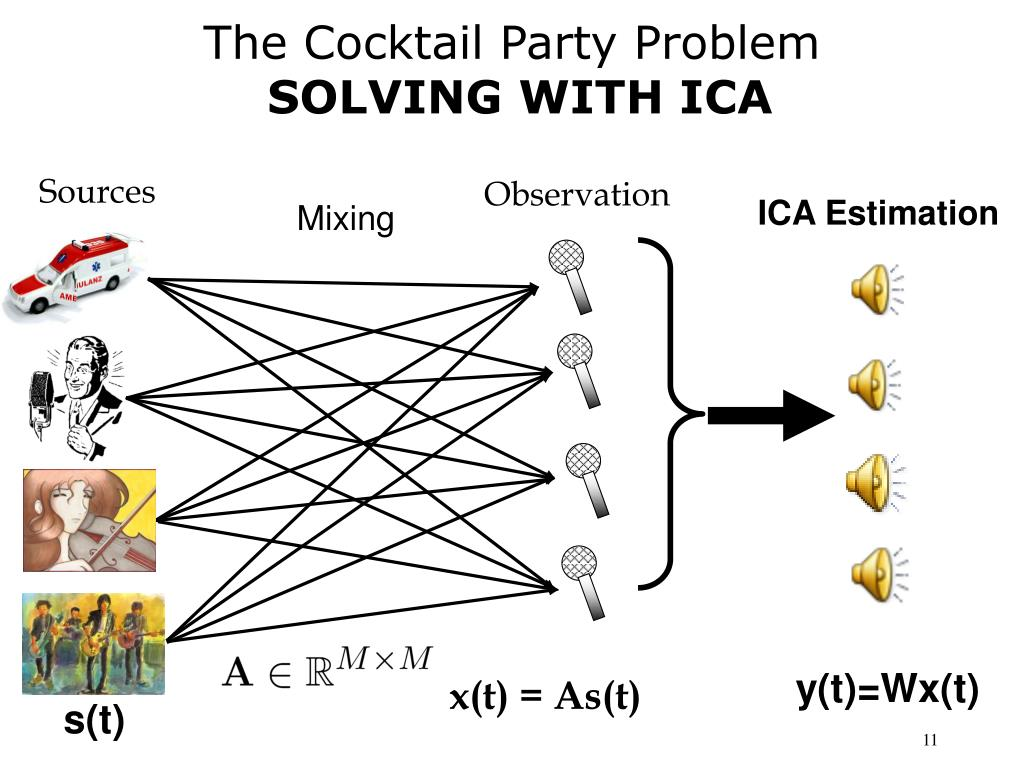
\includegraphics[width=\linewidth]{the cocktail party problem.jpg}
        \caption{Various Sources Mixing to Form Observation}
    \end{subfigure}
    \hfill
    \begin{subfigure}{0.45\textwidth}
        \centering
        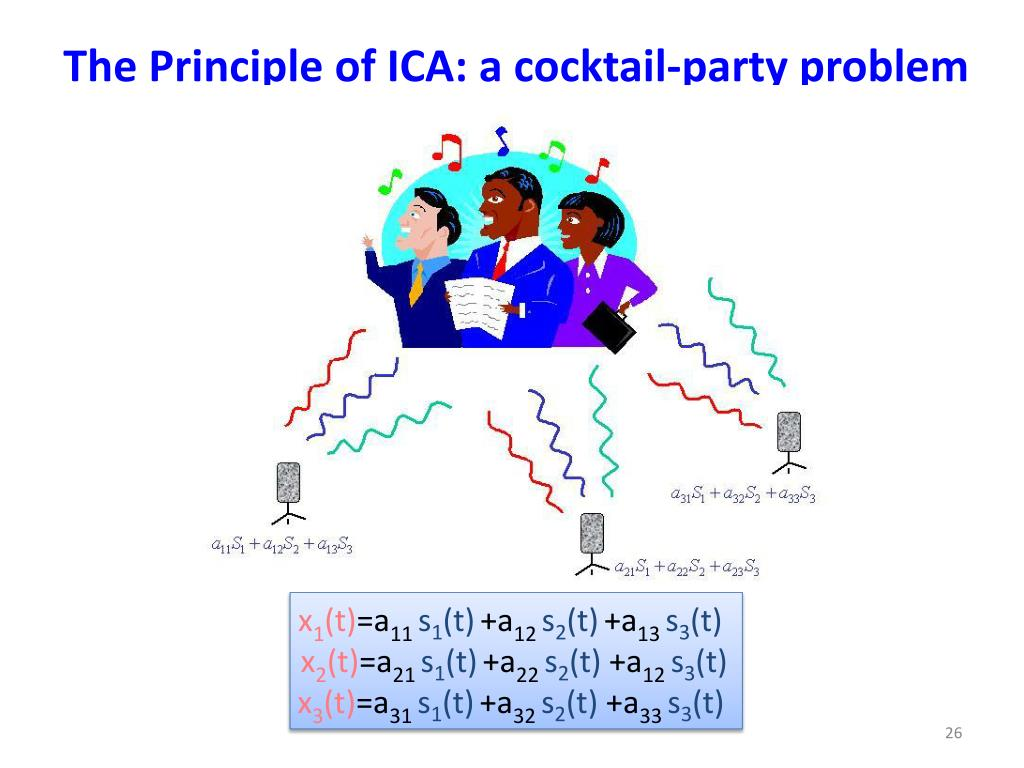
\includegraphics[width=\linewidth]{cocktail party prob.jpg}
        \caption{Principle of ICA}
        \end{subfigure}

    \caption{Images side by side}
\end{figure}

% =========================
\section*{Unmixing Model}
We seek an unmixing matrix $\mathbf{W}$ which give the recovered independent sources $\mathbf{y(t) = y_i}$.

\[
\mathbf{y_i} = \mathbf{W}.\x
\]

so,

\[
\mathbf{y_i} = \begin{bmatrix}
    w_{11} x_1 + \dots + w_{1n}x_n \\
    w_{21}x_1 + \dots + w_{2n} x_n \\
    \vdots \\
    w_{m1}x_1 + \dots + w_{mn}x_n
\end{bmatrix}
\]

Where $\mathbf{W}$ = Unmixing matrix and $\x$ = Observed values.

\[\mathbf{W} = \begin{bmatrix}
    w_{11} & w_{12} & w_{13} \\
    w_{21} & w_{22} & w_{23}\\
    w_{31} & w_{32} & w_{33}\\
\end{bmatrix} \]

The number of recovered sources $m$ cannot be larger than the number of observations n. 

From linear algebra, we can write $\mathbf{y} = \mathbf{W}.\x$ as $\mathbf{y} = \mathbf{W^T}\x$. 
% =========================
\section*{Projection of Observed Data}

We know that given an unknown mixing matrix $A$ and latent sources $s$, our observation is $\x = A . s$ \\

To recover the independent and maximally non-Gaussian components, we attempt unmixing.

\begin{align*}
\mathbf{y} &= \mathbf{W^T}\x \\
\mathbf{y} &= \mathbf{W^T} A s \\
\mathbf{y} &= (A^T \mathbf{W})^T s \\
\mathbf{y} &= z^Ts
\end{align*}

As a linear combination of $s_i$, $\mathbf{y}$ is more Gaussian than any $s_i$. To be maximally non-Gaussian, $\mathbf{y}$ must be equaly to one $s_i$. \\

Finding the first unmixing vector $\mathbf{W}$ to maximize the non-Gaussianity of $\mathbf{W^T}\x$ identifies the first independent component. Similarly, finding the second unmixing vector  $\mathbf{V}$, orthogonal to $\mathbf{W}$, to maximize the non-Gaussianity of $\mathbf{V^T}\x$ identifies the second independent component and subsequent independent components are identified by repeating the algorithm until it equals the number of observations.

% =========================
\section*{Central Limit Theorem}
The Central Limit Theorem states that a sum or linear combination of a large number of independent random variables tends toward a Gaussian distribution, regardless of the original distributions of those variables. In context of ICA, this means that when independent non-Gaussian sources $s_3, s_2, …, s_n$ are linearly mixed, the resulting mixture $\mathbf{y} = \mathbf{W^T}\x = \mathbf{z^T}s$ is more Gaussian than any individual source $s_i$. 

Meaning, Linear combinations of independent 'non-Gaussian' sources are more 'Gaussian' than the original sources.

\begin{figure}[h]
    \centering
    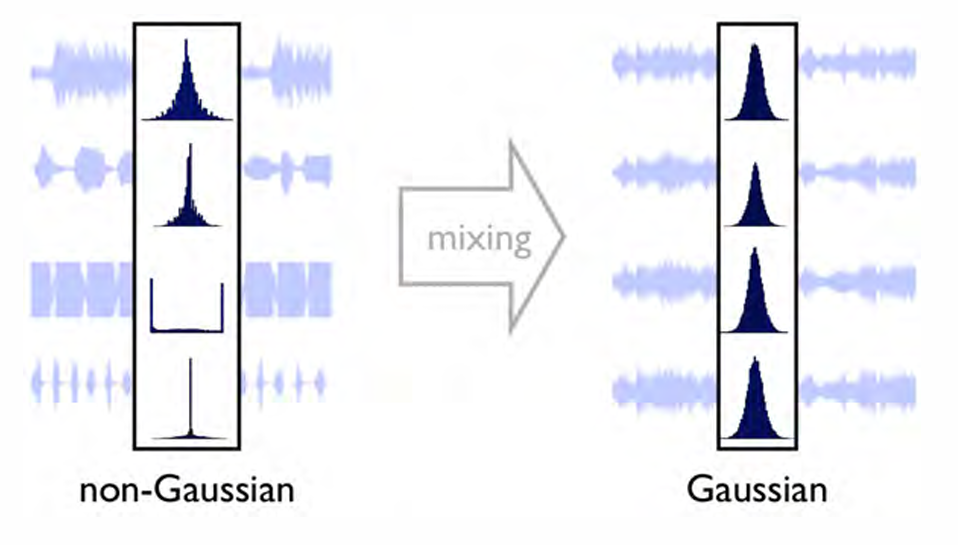
\includegraphics[width=1\linewidth]{Gaussian Mixtures.png}
    \caption{Mixtures become more Gaussian}
    \label{fig:placeholder}
\end{figure}

% =========================
\section*{Measures of Non-Gaussianity}
To use non-Gaussianity in ICA estimation, we must have a quantitative measure of non-Gaussianity of a random variable, say $y$. Non-Gaussianity can be measured through \textbf{Kurtosis} and \textbf{Negentropy}.

\subsection*{Kurtosis}
Kurtosis is a statistical measure that describes the shape of a data distribution and gives a clearer picture of how spread out or peaked the data really is beyond just the mean and variance.

The kurtosis of $y$ can be given as:
\[
Kurt(y) = \dfrac{E[(y-\mu)^4]}{\sigma^4}
\]

Since we work with centered data in ICA, $\mu =0$ and $\sigma^2 = 1$.

so,

\begin{align*}
   Kurt(y) &= \dfrac{E[y^4]}{(E[y^2])^2} = \dfrac{E[y^4]}{1} = E[y^4]
\end{align*}

Excess Kurtosis can be defined as:
\[
Kurt(y) = E[y^4] - 3(E[y^2])^2
\]

We assume that $y$ has been normalized so that its variance is equal to one. Then the right hand-side simplifies to $Kurt(y) = E[y^4] - 3$.

For a Gaussian $y$, $E[y^4] = 3(E[y^2])^2$. Therefore, kurtosis is zero for a Gaussian random variable. For non-Gaussian random variables, kurtosis is nonzero.

Kurtosis can be both positive or negative. Random variables that have a positive kurtosis are referred as supergaussian and those which have a negative kurtosis are referred to as subgaussian. In statistical literature, the same is referred as the terms 'leptokurtic' and 'platykurtic' respectively.\\

\textbf{Drawback of kurtosis:} \\
Kurtosis is not a robust measure of non-Gaussianity as it is sensitive to outliers. A single erroneous or irrelevant observation may produce an inaccurate interpretation.

\subsection*{Negentropy}
Negentropy is more robust than kurtosis but computationally complicated. The entropy of a random variable is related to the information that the observation of the variable gives. The more random or unpredictable and unstructured a variable is, the larger is its entropy.

The entropy of a random vector $y$ with density $p_y(\eta)$ is defined as:
\[
H(y) = - \int p_y(\eta) log p_y(\eta)d\eta
\]

A Gaussian variable has the largest entropy among all random variables of equal variance, suggesting that Gaussian distribution is the "most random" or the least structured of all distributions.

Negentropy can be defined as:
\[
J(y) = H(y_{gauss}) - H(y)
\]

Where $y_{gauss}$ = Gaussian random variable

Negentropy is always non-negative and it is zero only and only if $y$ has a Gaussian distribution.

\textbf{Approximation of Negentropy:}
\[
J(y) \approx \dfrac{1}{12}E[y^3]^2 + \dfrac{1}{48}Kurt(y)^2
\]

\textbf{Note:} This approximation is based on cumulants and still depends on kurtosis, meaning it retains some sensitivity to outliers. In practice, FastICA uses a more robust approximation
\[
J(y) \approx [\mathbf{E}[\mathbf{g}(y)] - \mathbf{E}[\mathbf{g}(z)]]^2
\]

Where $z =$ standard Gaussian random variable and $\mathbf{g}$ is a smooth non-linear function.
% =========================
\section*{Preprocessing}

\subsection*{Centering}
Observations $\x$ must have zero mean. This can be done by subtracting the mean from the original data.
\[
\tilde \x \leftarrow \x_{ori} - \mu
\]

\subsection*{Whitening}
Whitening's goal is to linearly transform the observed signals $\x$ in a way that potential correlations between the signals are removed and their variances equal unity. As a result, the covariance matrix of the whitened signals will be equal to unity. 

Given a random vector $\tilde \x$ with $n$ elements, we have to find a linear transformation $\mathbf{V_{PCA}}$ into another vector $\mathbf{z}$ such that
\[
\mathbf{z} = \mathbf{V_{PCA}}\tilde \x
\]

The PCA whitening matrix is given as:
\[
\mathbf{V_{PCA}} = \mathbf{D}^{-\dfrac{1}{2}} \mathbf{E^T}
\]

Where $\mathbf{E} = (e_1, e_2,\dots e_n)$ is the matrix whose columns are unit-norm eigenvectors of the covariance matrix $\mathbf{C_\x} = \mathbf{E}[\x \x^T] $ and $\mathbf{D} = diag(d_1, d_2, \dots d_n)$ is the diagonal matrix of the eigenvalues of $\mathbf{C}$.

$\mathbf{E^T}\x$ rotates the data and $\mathbf{D}^{-\dfrac{1}{2}}$ rescales each axis.

It is derived from 
\[\mathbf{C} = \mathbf{E}[\tilde \x \tilde \x^T] = \mathbf{EDE^T}\]

After whitening,
\[\mathbf{E}[\mathbf{zz^T}] = \mathbf{I}\]

FastICA implementations typically use PCA whitening internally.

\section*{FastICA Algorithm}
Recall that our goal is $\mathbf{y} = \mathbf{W^T}\x$. \\

\textbf{Step 1:} Choose some direction $\mathbf{W}$. \\

\textbf{Step 2:} Project data onto it.\\

\textbf{Step 3:} Check how non-Gaussian the result is.\\

\textbf{Step 4:} Improve $\mathbf{W}$.\\

\textbf{Step 5:} Repeat until $\mathbf{W_{new}} = \mathbf{W}$ i.e. $\mathbf{W}$ no longer changes. \\

\textbf{Fixed-Point Iteration (Update Rule):}
\[
\mathbf{W_{new}} = \mathbf{E}[\x \mathbf{g}(\mathbf{W^T}\x)] - \mathbf{E}[\mathbf{g'}(\mathbf{W^T}\x)] \mathbf{W}
\]

Where
$\mathbf{g}(u) = \tanh(u)$ and $\mathbf{g'}(u) = 1 - \tanh^2(u)$
\\

After updating, de-correlate and normalize $\mathbf{W}$.
\[
\mathbf{W_{new}} = \mathbf{W_{new}} -\sum_{j=1}^{new-1}(\mathbf{W_{new}}^T\mathbf{W}_j) \mathbf{W}_j
\]

Normalization:
\[
\mathbf{W_{new}} \leftarrow \dfrac{\mathbf{W_{new}}}{|| \mathbf{W_{new}} ||}
\]
Repeat until convergence, defined as:
\[
| \mathbf{W_{new}}^T \mathbf{W}| > 1 - \epsilon
\]

Where $\epsilon$ is a small tolerance ($10^{-4}$).
\end{document}